%%%%%%%%%%%%%%%%%%%%%%%%%%%%%%%%%%%%%%%%%%%%%%%%%%%%%%%%%%%%%%%%%%%%%%%%%%%%%%%%%%%%%%%
%%%%%%%%%%%%%%%%%%%%%%%%%%%%%%%%%%%%%%%%%%%%%%%%%%%%%%%%%%%%%%%%%%%%%%%%%%%%%%%%%%%%%%%
% 
% This top part of the document is called the 'preamble'.  Modify it with caution!
%
% The real document starts below where it says 'The main document starts here'.

\documentclass[12pt]{article}
\usepackage{graphicx}
\usepackage{float}
\usepackage{amssymb,amsmath,amsthm}
\usepackage[top=1in, bottom=1in, left=1.25in, right=1.25in]{geometry}
\usepackage{fancyhdr}
\usepackage{enumerate}
\usepackage{listings}
% Comment the following line to use TeX's default font of Computer Modern.
\usepackage{times,txfonts}

\newtheoremstyle{homework}% name of the style to be used
  {18pt}% measure of space to leave above the theorem. E.g.: 3pt
  {12pt}% measure of space to leave below the theorem. E.g.: 3pt
  {}% name of font to use in the body of the theorem
  {}% measure of space to indent
  {\bfseries}% name of head font
  {:}% punctuation between head and body
  {2ex}% space after theorem head; " " = normal interword space
  {}% Manually specify head
\theoremstyle{homework} 

% Set up an Exercise environment and a Solution label.
\newtheorem*{exercisecore}{Exercise \@currentlabel}
\newenvironment{exercise}[1]
{\def\@currentlabel{#1}\exercisecore}
{\endexercisecore}

\newcommand{\localhead}[1]{\par\smallskip\noindent\textbf{#1}\nobreak\\}%
\newcommand\solution{\localhead{Solution:}}

%%%%%%%%%%%%%%%%%%%%%%%%%%%%%%%%%%%%%%%%%%%%%%%%%%%%%%%%%%%%%%%%%%%%%%%%
%
% Stuff for getting the name/document date/title across the header
\makeatletter
\RequirePackage{fancyhdr}
\pagestyle{fancy}
\fancyfoot[C]{\ifnum \value{page} > 1\relax\thepage\fi}
\fancyhead[L]{\ifx\@doclabel\@empty\else\@doclabel\fi}
\fancyhead[C]{\ifx\@docdate\@empty\else\@docdate\fi}
\fancyhead[R]{\ifx\@docauthor\@empty\else\@docauthor\fi}
\headheight 15pt

\def\doclabel#1{\gdef\@doclabel{#1}}
\doclabel{Use {\tt\textbackslash doclabel\{MY LABEL\}}.}
\def\docdate#1{\gdef\@docdate{#1}}
\docdate{Use {\tt\textbackslash docdate\{MY DATE\}}.}
\def\docauthor#1{\gdef\@docauthor{#1}}
\docauthor{Use {\tt\textbackslash docauthor\{MY NAME\}}.}
\makeatother

% Shortcuts for blackboard bold number sets (reals, integers, etc.)
\newcommand{\Reals}{\ensuremath{\mathbb R}}
\newcommand{\Nats}{\ensuremath{\mathbb N}}
\newcommand{\Ints}{\ensuremath{\mathbb Z}}
\newcommand{\Rats}{\ensuremath{\mathbb Q}}
\newcommand{\Cplx}{\ensuremath{\mathbb C}}
%% Some equivalents that some people may prefer.
\let\RR\Reals
\let\NN\Nats
\let\II\Ints
\let\CC\Cplx

%%%%%%%%%%%%%%%%%%%%%%%%%%%%%%%%%%%%%%%%%%%%%%%%%%%%%%%%%%%%%%%%%%%%%%%%%%%%%%%%%%%%%%%
%%%%%%%%%%%%%%%%%%%%%%%%%%%%%%%%%%%%%%%%%%%%%%%%%%%%%%%%%%%%%%%%%%%%%%%%%%%%%%%%%%%%%%%
% 
% The main document start here.

% The following commands set up the material that appears in the header.
\doclabel{Stat 300: Homework 10}
\docauthor{Stefano Fochesatto}
\docdate{\today}

\begin{document}

\begin{exercise}{Bootstrap} Bootstrapping is often needed when we have an unusual statistic and don't know its
   standard error (Ch. 6) or else when we can't trust the central limit theorem to help us 
  (by allowing us, in Ch. 7, to use plus or minus 2 standard errors to get a confidence interval)
  and need to find the 95\% confidence interval directly.  
    Suppose we have collected the following data from an exponential distribution:  
    (4.1, 15.2, 14.3, 3.1, 25.8, 9.6, 4.1, 14.7, 4.9, 8.7)
    and we want to estimate the rate $(1/\mu)$ with the estimator $1/\overline{x}$.  
    I have know idea what the standard error is of that estimator.  
    Calculate the estimate for this data and then use bootstrapping to get an estimate of the standard error.
    (Hint:  follow the example from class\\

    \solution 
    Using r we can create a large Bootstrap sample to estimate $(1/\mu)$, calculate the $95\%$ confidence interval
    and standard error. We end up with a sample estimator of  $1/\overline{x} = .1002935$, confidence interval of 
    $(0.06756757, 0.1517451)$ and a standard error of $.02161504$.\\

    \textbf{Console:}
    \begin{center}
    \lstinputlisting{bootstrap.txt}
    \end{center}
    \begin{figure}[H]
      \caption{Histogram of Bootstrap sample}
      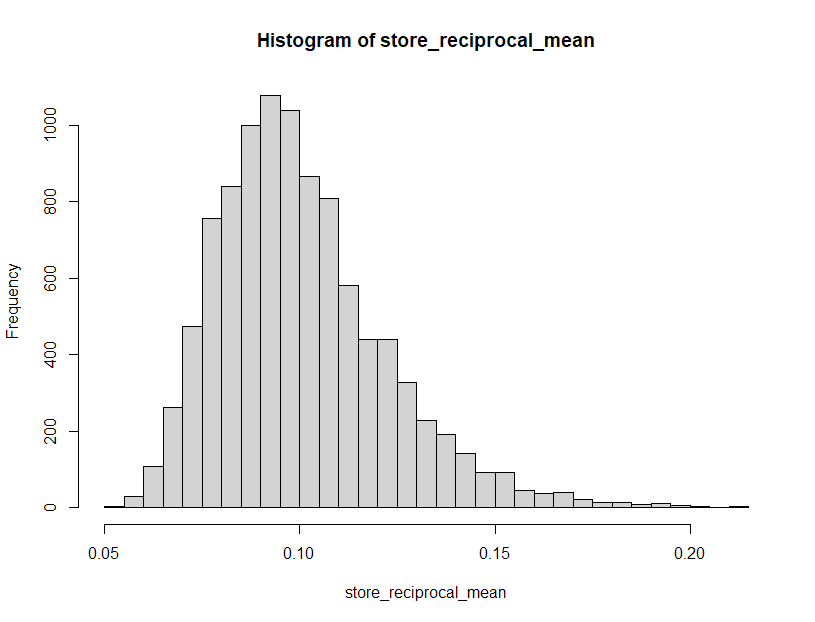
\includegraphics[width = \textwidth]{bootstrap.png}  
      \centering
    \end{figure}

\end{exercise}
\vspace{.5in}


\begin{exercise}{7.4} A  CI  is  desired  for  the  true  average  stray-load  loss  $\mu$ (watts)  for  a 
   certain  type  of  induction  motor  when  the  line current is held at 10 amps for a speed of 1500 rpm.
    Assume that stray-load loss is normally distributed with $\sigma = 3.0$\\
    \begin{enumerate}
      \item Compute a $95\%$ CI for $\mu$ when $n = 25$ and $\overline{x} = 58.3$.\\
      \solution Computing the $95\%$ CI from the definition,
      \begin{equation*}
        95\% CI = (\overline{x} - z_{.025}\dfrac{\sigma}{\sqrt{n}}, \overline{x} + z_{.025}\dfrac{\sigma}{\sqrt{n}})
      \end{equation*}
      \begin{equation*}
        95\% CI = (58.3 - 1.96 \dfrac{3.0}{\sqrt{25}}, 58.3 + 1.96 \dfrac{3.0}{\sqrt{25}}),
      \end{equation*}
      \begin{equation*}
        95\% CI = (57.1, 59.5).
      \end{equation*}
      \vspace{.25in}
    


      \item Compute a $95\%$ CI for $\mu$ when $n = 100$ and $\overline{x} = 58.3$.\\
      \solution Computing the $95\%$ CI from the definition,
      \begin{equation*}
        95\% CI = (58.3 - 1.96 \dfrac{3.0}{\sqrt{100}}, 58.3 + 1.96 \dfrac{3.0}{\sqrt{100}}),
      \end{equation*}
      \begin{equation*}
        95\% CI = (57.7, 58.9).
      \end{equation*}
      \vspace{.25in}
    


      \item Compute a $99\%$ CI for $\mu$ when $n = 100$ and $\overline{x} = 58.3$.\\
      \solution Computing the $99\%$ CI from the definition and $z_{.005} = 2.58$,
      \begin{equation*}
        99\% CI = (58.3 -  2.58 \dfrac{3.0}{\sqrt{100}}, 58.3 + 2.58\dfrac{3.0}{\sqrt{100}}),
      \end{equation*}
      \begin{equation*}
        99\% CI = (57.5, 59.1).
      \end{equation*}
      \vspace{.25in}


      \item Compute a $82\%$ CI for $\mu$ when $n = 100$ and $\overline{x} = 58.3$.\\
      \solution Computing the $82\%$ CI from the definition and $z_{.09} = 1.34$,
      \begin{equation*}
        82\% CI = (58.3 - 1.34\dfrac{3.0}{\sqrt{100}}, 58.3 + 1.34\dfrac{3.0}{\sqrt{100}}),
      \end{equation*}
      \begin{equation*}
        82\% CI = (57.9, 58.7).
      \end{equation*}
      \vspace{.25in}

      \item How large must $n$ be if the width of the $99\%$ CI for $\mu$ is to be 1.0?
      \solution Solving for $n$ by the definition of a $99\%$ CI with width $w = 1$,
      \begin{align*}
        w &= 2z_{.005}\dfrac{\sigma}{\sqrt{n}},\\
        n &= (2z_{.005}\dfrac{\sigma}{w})^2.
      \end{align*}
      Substituting and solving for $n$,
      \begin{equation*}
        n = (2(2.58)\dfrac{3.0}{1})^2 = 239.62.
      \end{equation*}

    \end{enumerate}
\end{exercise}
\vspace{.5in}













\begin{exercise}{7.10} A random sample of $n = 15$ heat pumps of a certain type yielded the
following observations on lifetime (in years) \dots Assume tha the lifetime distribution is exponential
and use an argument parallel to that of example 7.5 to obtain a $95\%$ CI for the expected average lifetime.\\

\solution Consider the random variable $h(X_1,X_2,\dots,X_{15}) = 2\lambda\sum X_i$. Following the 
example we know that this variable is a chi-square distribution with $2n = 2(15) = 30$ degrees of freedom. From 
Table $A.7$ we know the critical values $\chi^2_{.975,30} = 16.791$ and $\chi^2_{.025,30} = 46.976$. From the example we get 
that the confidence interval for the parameter $\mu = 1/\lambda$ and where $\sum x_i = 63.2$ from our given data,
\begin{equation*}
  95\% = (\dfrac{2\sum x_i}{16.791}, \dfrac{2\sum x_i}{46.976}) = (2.69, 7.53).
\end{equation*}
\end{exercise}
\vspace{.5in}






\begin{exercise}{7.16} The  alternating  current  (AC)  breakdown  voltage  of  an  insulating  liquid  indicates  its
dielectric  strength\dots\\
\begin{enumerate}
  \item Construct a boxplot of data and comment on any interesting features.\\
  \solution The following is a boxplot generated in $r$
  \begin{figure}[H]
    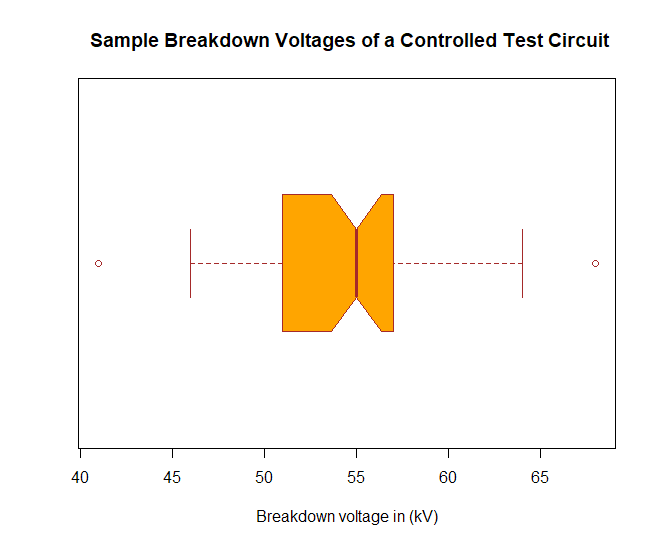
\includegraphics[width = .75\textwidth]{Voltages.png}  
    \centering
  \end{figure}
  Looking at the box plot we can see that the data is fairly, normally distributed. There is a little bit of a left skew
  but we also have outliers on either side of the median. We can also see this looking at the five number summary,
  \begin{equation*}
  \begin{bmatrix}
    Min. && 1st Qu. && Median && 3rd Qu. && Max.\\ 
    41 && 51 && 55 && 57 && 68
  \end{bmatrix}
  \end{equation*}
  \vspace{.25in}

  \item Calculate  and  interpret  a  $95\%$  CI  for  true  average  breakdown voltage $\mu$.\
   Does it appear that $\mu$ has been precisely estimated? Explain.\\
   \solution Computing the sample mean and the variance/standard deviation of the sample mean in order to calculate the 
   large-sample confidence interval.
   \textbf{Console:}
   \begin{center}
   \lstinputlisting{samplemean.txt}
   \end{center}
   Since we are calculating the $95\%$ CI we use $x_{0.025} = 1.96$ we get the following,
   \begin{equation*}
    95\% = (54.7083 - 1.96 \dfrac{5.2306}{\sqrt{48}}, 54.7083 + 1.96 \dfrac{5.2306}{\sqrt{48}})
   \end{equation*}
   \begin{equation*}
    95\% = (53.2285, 56.1881)
   \end{equation*}
   With a margin of error around 1.5m, $\overline{x}$ seems to be a relatively precise estimate for $\mu$.
   \vspace{.25in}



\item  Suppose  the  investigator  believes  that  virtually  all  values of breakdown voltage are between 
40 and 70. What sample size would be appropriate for the 
$95\%$ CI to have a width of 2 kV (so that $\mu$ is estimated to within 1 kV with $95\%$ confidence)?\\
\solution Solving for $n$ with a new width for the confidence interval,
\begin{equation*}
  2 = 2(1.96) \dfrac{\sigma}{\sqrt{n}}.
\end{equation*}
Given what the investigator believes we can estimate the standard deviation $\sigma$ by taking the difference 
between the largest and smallest values and dividing it by 4,
\begin{equation*}
  \sigma \approx \dfrac{70-40}{4} = 7.5.
\end{equation*}
Using that we can solve for $n$,
\begin{equation*}
  n = (2(1.96) \dfrac{7.5}{2})^2 = 216.09.
\end{equation*}
A sample size above 220 would likely be the safest bet. 
  \end{enumerate}
\end{exercise}
\vspace{.5in}




\begin{exercise}{7.20} TV  advertising  agencies  face  increasing  challenges  in 
reaching audience members because viewing TV programs via  digital  streaming  is  gaining  in  popularity\dots\\
\begin{enumerate}
  
  \item Calculate  and  interpret  a  confidence  interval  at  the  $99\%$ confidence level for the proportion 
  of all adult Americans  who  watched  streamed  programming  up  to that point in time.\\
  \solution Given our point estimation for $p$, $\hat{p} = .53$ and our sample size $n = 2343$. Using Proposition 7.11 we can calculate the 
  $99\%$ confidence level with critical point $z_{.005} = 2.575$ for the population proportion,
  \begin{equation*}
    99\% CI = (.53 - 2.575\sqrt{\dfrac{.53(1 - .53)}{2343}}), (.53 + 2.575\sqrt{\dfrac{.53(1 - .53)}{2343}}),
  \end{equation*}
  \begin{equation*}
    99\% CI = (.5034, .5566).
  \end{equation*}
  \vspace{.25in}


  \item What sample size would be required for the
   width of a $99\%$ CI to be at most .05 irrespective of the value of $\hat{p}$?\\

   \solution When $\hat{p}$ is unknown we approximate with $\hat{p} = .50$. solving for $n$ using Proposition 7.11 with 
   a given width of $.5$,
   \begin{align*}
     .05 &= 2(2.575)\sqrt{\dfrac{.50(1 - .50)}{n}},\\
     .05 &= 2(2.575)\sqrt{\dfrac{.25}{n}},\\
     n &= 2(2.575)^2\dfrac{.25}{.05^2},\\
     n &= 1326.125.
   \end{align*}
Therefore we would need a sample size of approximately $n = 1327$ to get a width of $.05$ in an $99\%$ CI.
\end{enumerate}
\end{exercise}
\vspace{.5in}



\begin{exercise}{7.32}  According to the article Fatigue\dots Calculate and interpret a confidence interval 
  at the $99\%$ confidence level for the true average number of cycles to break.\\
\solution Given that $n = 20$, we have a sample mean of $\overline{x} = 1584$ with a standard deviation of $s = 607$
all we have to do is find the critical value at $t_{.005}$ for a $t$ distribution with $19$ degrees of freedom. Through table $A.5$ we get that 
$t_{.005,19} =2.861$ and by Proposition 7.15 we get that the confidence interval is,
\begin{equation*}
  99\% CI = (1584 - 2.861 \dfrac{607}{\sqrt{20}}),1584 + 2.861 \dfrac{607}{\sqrt{20}} ),
\end{equation*}
\begin{equation*}
  99\% CI = (1195.68, 1972.32).
\end{equation*}
\end{exercise}
\vspace{.5in}














\begin{exercise}{7.36} A normal probability plot of the $n = 26$ observations on escape  time  given  in  Exercise  36  of 
  Chapter  1  shows  a  substantial  linear  pattern;  the  sample  mean  and  sample  standard deviation are 370.69 and 24.36, 
  respectively.\\
  \begin{enumerate}
    \item  Calculate  an  upper  confidence  bound  for  population mean escape time using a confidence level of $95\%$\\
    \solution To calculate the upper bound for the $95\%$ confidence interval we must determine the critical value at $t_{.025}$ for a $t$ distribution with $25$ degrees of freedom.
    Through table $A.5$ we get that 
    $t_{.025,25} = 1.708$ and by Proposition 7.15 we get that the upper bound is,
    \begin{equation*}
      370.69 + 2.861 \dfrac{24.36}{\sqrt{26}} = 378.84.
    \end{equation*}

    \item  Calculate  an  upper  prediction  bound  for  the  escape  time of a single additional worker using a prediction level of $95\%$. 
    How does this bound compare with the confidence bound of part (a)?\\
    \solution Using the same critical value at $t_{.025}$ we can calculate the upper bound of the prediction interval by Proposition 7.16
    \begin{equation*}
      370.69 + 2.861(24.36) \sqrt{1 + \dfrac{1}{26}} = 42.39.
    \end{equation*}

  \end{enumerate}

\end{exercise}

\end{document}